% Document settings
\documentclass[11pt]{article}
\usepackage[margin=1in]{geometry}
\usepackage{graphicx}
\usepackage{multirow}
\usepackage{setspace}
\usepackage{amsmath,amssymb,gensymb,epsfig, epstopdf}
\usepackage{xcolor}
\pagestyle{plain}
\setlength\parindent{0pt}
\setlength{\parskip}{1em}

\begin{document}

% Header
\textbf{Nitin Kapania} \\
\textbf{Relative Dynamics for Bicycle Model} \\ 

\section{Problem Formulation}
Consider an autonomous vehicle driving at a constant highway speed on a straight road, attempting to avoid a static obstacle while staying within the road boundaries. This maneuver will require high vehicle lateral acceleration. 

\begin{center}
 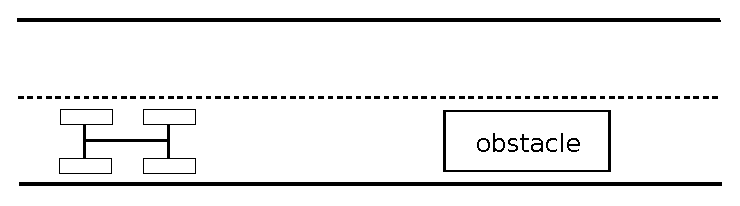
\includegraphics[width=.6\textwidth]{Images/problemDefinition.eps}
\end{center}


\section{Tracker Dynamics}

The dynamics of the vehicle in this situation can be described with the following four states:

\begin{equation} 
s = [e \hspace{1 mm} \Delta\Psi \hspace{1 mm}  r \hspace{1 mm} \hspace{1 mm} \beta]^T
\end{equation}

where $e$ is the lateral deviation from the desired path, $\Delta\Psi$ is the heading deviation from the desired path, $r$ is the vehicle yaw rate, $\beta$ is the vehicle sideslip (see below). Note that $x$ is distance along the path and is needed to determine distance from the obstacle, but is not relevant for the lateral path tracking.  

 \begin{center}
   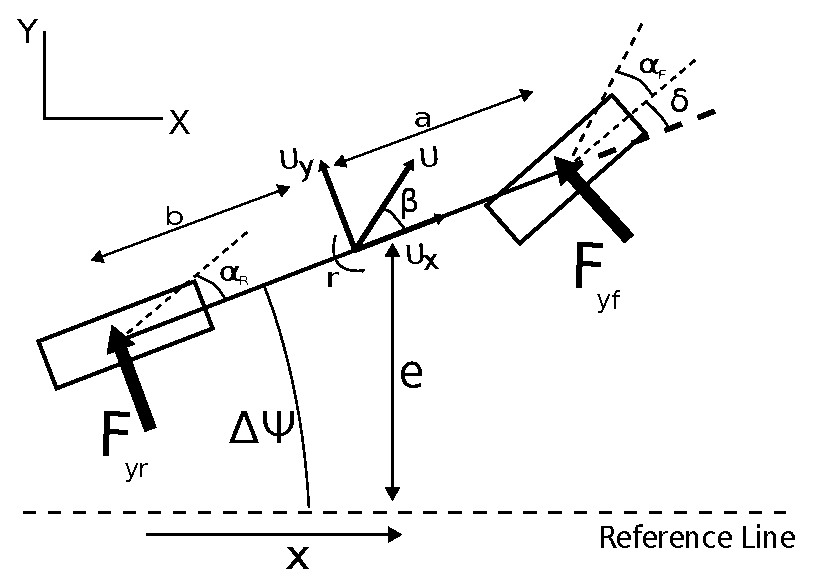
\includegraphics[width=.6\textwidth]{Images/bikeModel2.eps}
 \end{center}

For a vehicle attempting a highly dynamic maneuver, the force generated by the tires begins to saturate, creating nonlinear dynamics. The dynamics are defined by the following ODEs:

\begin{subequations}
\label{eq:bm}
\begin{align}
	\dot{\beta} &= \frac{F_\mathrm{yf}\cos{\delta}+F_\mathrm{yr}}{mU_x} - r \label{eq:bm1}\\
	\dot{r} &= \frac{aF_\mathrm{yf}\cos{\delta} - bF_\mathrm{yr}}{I_z} \label{eq:bm2} \\
	\dot{e} &= U_x\sin{\Delta\Psi} + U_y\cos{\Delta\Psi} \label{eq:bm3} \\
	\Delta\dot{\Psi} &= r \label{eq:bm4} \\
	%\dot{x} &= \frac{U_x\cos\Delta\Psi - U_y\sin(\Delta\Psi)}{1 - \kappa e}
\end{align}
\end{subequations}

The front and rear tire forces $F_{yf}$ and $F_{yr}$ are functions of the tire slip angles, given by:

\begin{equation}
\alpha_F = \frac{ U_y + ar }{U_x} - \delta
\end{equation}

\begin{equation}
\alpha_R = \frac{U_y - br}{U_x}
\end{equation}

Note that each tire has separate cornering stiffnesses $C_f$ and $C_r$ and normal forces $F_{zf}$ and $F_{zr}$

\begin{eqnarray}
\label{eqn:fiala}
	F_\mathrm{y}&=&\begin{cases} -C_{\alpha}\tan\alpha + \frac{C_{\alpha}^2}{3\mu F_\mathrm{z}} |\tan\alpha| \tan\alpha - \frac{C_{\alpha}^3}{27\mu^2F_\mathrm{z}^2}\tan^3\alpha,
\hspace{4mm}  |\alpha| < \arctan{\left(\frac{3\mu F_\mathrm{z}}{C_\alpha}\right)} \\ -\mu F_\mathrm{z}\text{sgn} \ \alpha, \hspace{62mm} \mathrm{otherwise} \end{cases}
\end{eqnarray}

The control input is the steer angle, $\delta$, which indirectly appears in the ODEs through the tire slip angle, then the tire force. Assume the following parameter set:
\newpage

\begin{table}[h]
\small
\begin{center}
\caption{Vehicle Parameters}\label{tb:params}
\begin{tabular}{lccc}
Parameter & Symbol & Value & Units \\\hline
Vehicle mass & $m$ & 1500 & kg \\
Yaw moment of inertia & $I_z$ & 2250 & $\mathrm{kg \cdot m}^2$\\
Front axle to CG & $a$ & 1.04 & m\\
Rear axle to CG & $b$ & 1.42 & m\\
Gravity acceleration & 9.81 & $m/s^2$ \\
Front cornering stiffness & $\mathrm{C}_\mathrm{F}$ & 8500 & $N$ \\
Rear cornering stiffness & $\mathrm{C}_\mathrm{R}$ & 6300 & $N$ \\
Tire road friction (both tires)  & $\mu$ & 1.0 & \\
Front normal force & $F_{zf}$ & 8560 & $\mathrm{N}$ \\
Rear normal force & $F_{zr}$ & 6275 & $\mathrm{N}$ \\ 
Vehicle Velocity & $U_x$ & 30 & m/s \\
\end{tabular}
\end{center}
\end{table}


\section{Planner Dynamics}


% \begin{center}
% 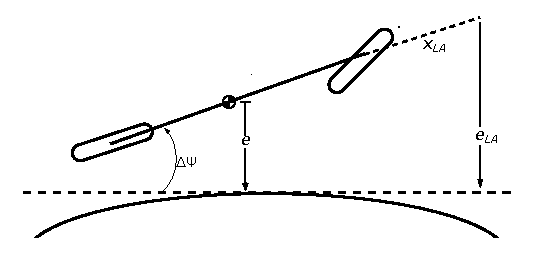
\includegraphics[width=.6\textwidth]{fig1.eps}
% \end{center}

While it is possible to run model-based online control with a fully nonlinear vehicle model, this is still an area
of active research focus. A simpler planning model is to assume no saturation of tire force as the vehicle turns - i.e.:

\begin{equation}
    F_y = - C\alpha
\end{equation} 

In this case, the vehicle dynamics can now be written as a linear dynamical system of the form:

\begin{equation}
\dot{s} = As + B\delta	
\end{equation}

where $A$ and $B$ are given by:

\begin{subequations}
\label{eqn:Amatrix}
\begin{align}
    \dot{x} &= Ax + B\kappa  \\
	A  &=  \begin{bmatrix}
   0 & U_\mathrm{x} & 0 & U_\mathrm{x} \\ 
   0 & 0 & 1 & 0 \\ 
   0  & 0  & -\frac{a^2C_\mathrm{F}+b^2C_\mathrm{R}}{U_\mathrm{x}I_\mathrm{z}} & \frac{bC_\mathrm{R} - aC_\mathrm{F}}{I_\mathrm{z}}  \\
   0  & 0  & \frac{bC_\mathrm{R}-aC_\mathrm{F}}{mU_\mathrm{x}^2}-1 & -\frac{C_\mathrm{F} + C_\mathrm{R}}{mU_\mathrm{x}}
  \end{bmatrix} \\
	B  &=[0 \hspace{2 mm} 0 \hspace{3 mm} \frac{aC_f}{I_z} \hspace{3 mm} \frac{C_f}{mU_x}]^T
\end{align}
\end{subequations}




\end{document}



